\documentclass[11pt,letterpaper]{article}
\usepackage[margin=0.72in]{geometry}
\usepackage{fontspec}
\setmainfont{Times New Roman}
\usepackage{amsmath,booktabs,array,graphicx,float,url}
\usepackage[hidelinks]{hyperref}
\usepackage{fancyhdr}
\pagestyle{fancy}\fancyhf{}
\lhead{Fund X: return-based due diligence}\rhead{11 November 2026}
\cfoot{\thepage}\renewcommand{\headrulewidth}{0.3pt}
\setlength{\headheight}{14pt}
\setlength{\parindent}{0pt}\setlength{\parskip}{5pt}
\setlength{\tabcolsep}{7pt}\renewcommand{\arraystretch}{1.15}
\newcommand{\subhead}[1]{\vspace{5pt}{\large\bfseries #1}\par}
\newcommand{\note}[1]{{\small #1\par}}
\begin{document}
\begin{center}
{\LARGE\bfseries Screening Chen--Zimmermann portfolios}\\[5pt]
{\large Assignment 9: results and implications for the paper}
\end{center}

\subhead{What the results show}
Monthly returns can tell an investor where to investigate, but a warning does not identify its cause and a quiet screen does not verify a record. This exercise tests warnings on published strategies, selection of strong historical performers, and the cost of stricter cutoffs.

Only \textbf{1 of 195} unmodified long--short portfolios triggers either conventional screen over January 2017--December 2025. Choosing the strongest performer does not consistently increase warnings. A stricter selection-based cutoff removes the one warning in the held-out 194-strategy cohort, but detects fewer deliberately altered records: \textbf{66/194 versus 120/194} under the specified three-month loss-recognition policy. Calibration has a measured detection cost.

\subhead{Data and the economic comparison}
The official October 2026 Chen--Zimmermann release contains 212 long--short factor series. Of these, 195 have all 108 observations in the common window; 194 also have complete 2005--2016 calibration histories. Data end in December 2025, so Fund X's 2026 returns are excluded from comparisons. No missing months are filled. The exact release is frozen for reproduction.

The long--short spread is the long portfolio's return minus the short portfolio's return. These are reconstructed stock-strategy returns, not live hedge-fund NAVs. All 195 strategies were published by 2016; the updated data and published-factor catalogue remain retrospective. Source returns exclude implementation and management costs; Fund X is reported net of fees.

\begin{center}
\begin{tabular}{llrrr}
\toprule
Weighting & Return & Bias & Normal & Either \\
\midrule
Original constructions & Long--short spread & 1 & 1 & 1 \\
Original constructions & Cash + spread & 3 & 4 & 4 \\
Forced value weighting & Long--short spread & 0 & 0 & 0 \\
Forced value weighting & Cash + spread & 0 & 0 & 0 \\
\bottomrule
\end{tabular}
\end{center}
\note{Each row has 195 portfolios. ``Either'' means bias ratio $>2$ or fitted-normal loss-count $p<0.05$. Original constructions use the source paper's portfolio weights; the alternative forces stock value weighting while retaining the original sorts.}

\begin{center}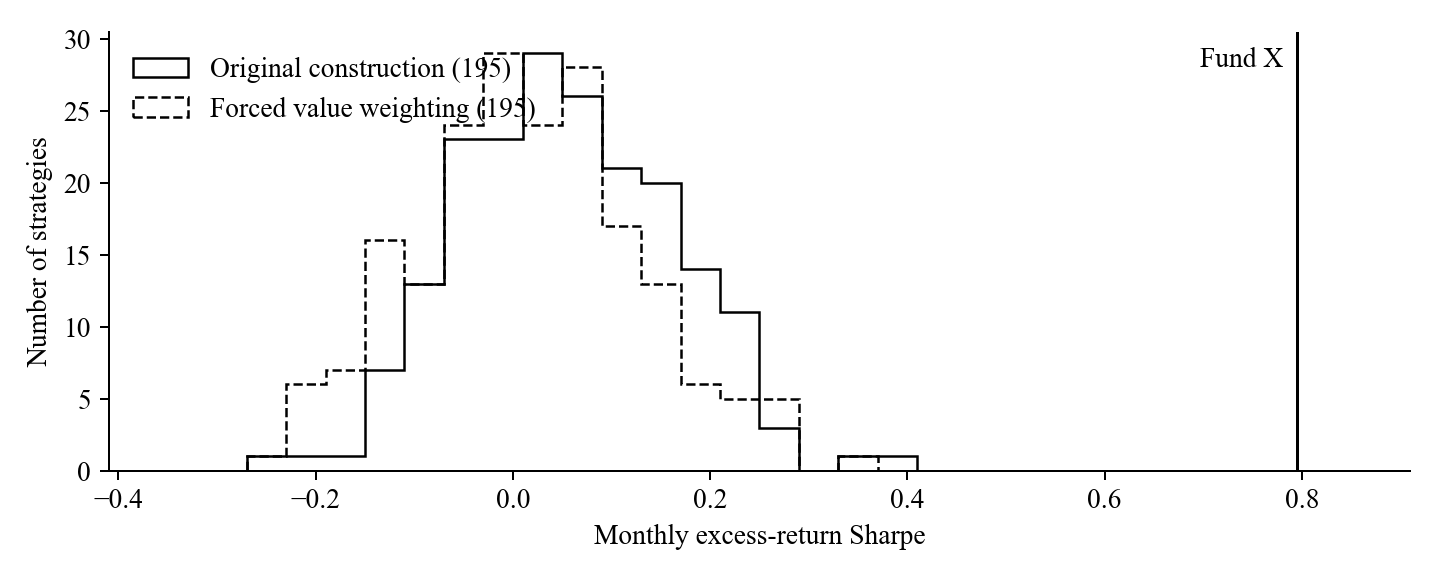
\includegraphics[width=0.93\linewidth]{figures/performance_support.png}\end{center}
\note{Monthly excess-return Sharpe ratios. Fund X is 0.796; the strongest individual original-construction factor is 0.406. The individual-factor panel therefore does not reproduce Fund X's performance range.}

\newpage
\subhead{1. Selecting a strong historical record}
The investor is assumed to review $K$ different strategies and choose the one with the highest realised excess-return Sharpe ratio over the same record being screened. This describes selection after seeing a track record; it is not an out-of-sample investment strategy. The 194 eligible names are kept fixed.

For each $K$, the calculation averages over every possible size-$K$ subset without drawing artificial fund histories. If rank $j$ is the $j$th strongest strategy, its chance of being selected is
\[
  w_j(K)=\frac{\binom{194-j}{K-1}}{\binom{194}{K}},
\qquad
  A(K)=\sum_j w_j(K)\,\mathbf 1\{\text{strategy }j\text{ warns}\}.
\]
Thus $K=1$ means a random strategy, while $K=194$ means the single strongest record in the whole cohort. Shared stocks and common market shocks do not invalidate this conditional subset calculation. Ties are resolved alphabetically.

\begin{center}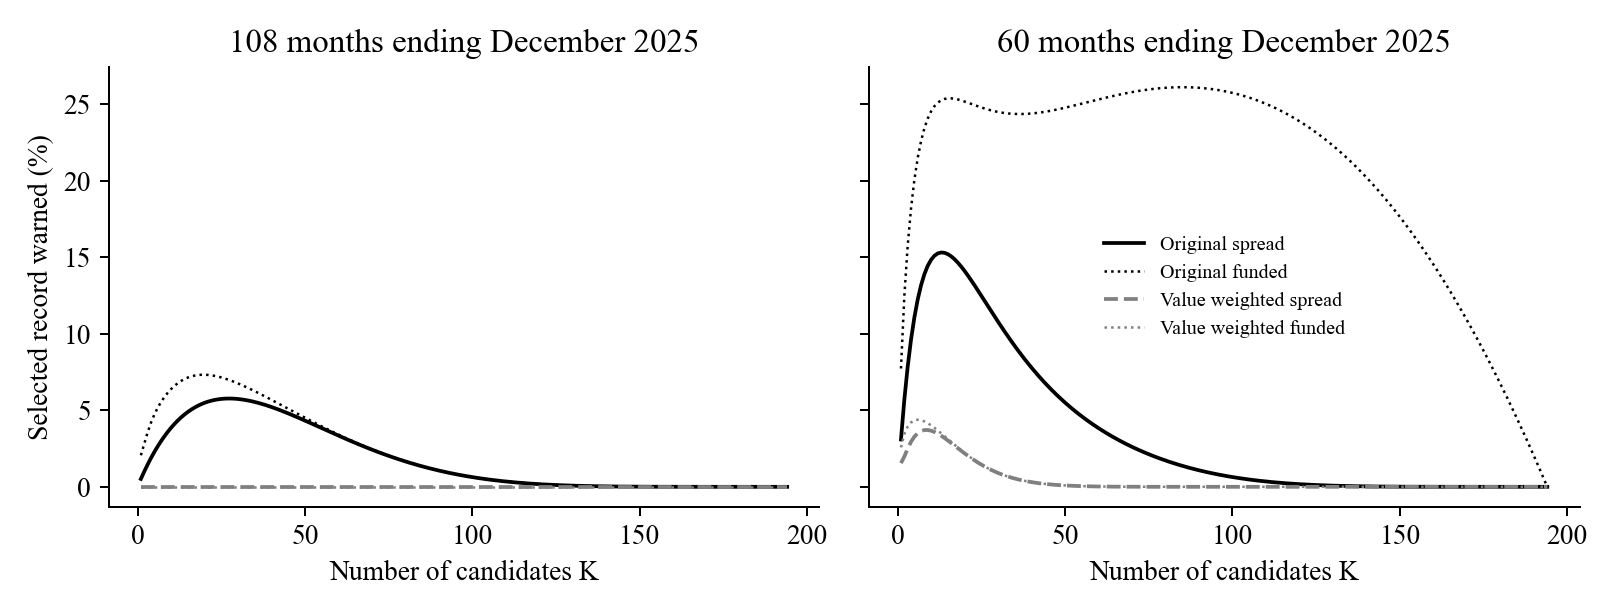
\includegraphics[width=\linewidth]{figures/selection_curves.png}\end{center}

For the original long--short spreads over 108 months, the conventional warning probability is \textbf{0.52\%} for a random name, \textbf{5.49\%} for the best of 20, and \textbf{0\%} for the best of all 194. The single flagged factor, Mom12mOffSeason, lies below the top of the Sharpe ranking. Its bias ratio is 2.28 and normal-count $p$ is 0.0217; its skewness is negative. It does not recreate Fund X's unusually high bias ratio and positive-skew pattern.

Shorter records show larger but uneven selection effects:
\begin{center}
\begin{tabular}{lrrr}
\toprule
60-month end & Random ($K=1$) & Best of 20 & Best of 194 \\
\midrule
2021 & 3.09\% & 7.61\% & 0.00\% \\
2022 & 1.03\% & 7.32\% & 0.00\% \\
2023 & 1.03\% & 0.27\% & 0.00\% \\
2024 & 1.55\% & 10.34\% & 100.00\% \\
2025 & 3.09\% & 14.11\% & 0.00\% \\
\bottomrule
\end{tabular}
\end{center}
\note{Original-construction spreads; either conventional screen. Each row is a different 60-month record. The five records overlap and are not independent trials.}

\textbf{Economic reading.} Searching across strategies can raise the chance of encountering a warning, but the effect depends on which strategies sit near the top and on the review window. It is not a general increasing relationship between performance and suspicious-looking returns. In 2024 the best full-pool record warns; in 2025 it does not. Forced value weighting produces fewer warnings, while adding cash interest matters particularly for low-volatility records.

\newpage
\subhead{2. A historical reference cutoff, and its limits}
The conventional bias ratio counts small gains relative to small losses:
\[
 B=\frac{\#\{0\le r_t\le s\}}{1+\#\{-s\le r_t<0\}},
\qquad
 D=T\Phi(-\bar r/s)-\#\{r_t<0\}.
\]
Here $s$ is sample standard deviation. Large $D$ means fewer losses than the fitted normal distribution predicts. The normal-count screen uses the lower binomial tail with fitted probability $\Phi(-\bar r/s)$. Since the probability is estimated from the same record and months may be dependent, this is a screening calculation, not an exact 5\% test. It is the paper's Gaussian adaptation, not the original pooled Bollen--Pool test.

To compare the two scores, each is converted to its percentile in complete development windows ending each December during 1980--2004. The combined score is the larger percentile. These percentiles are rankings, not $p$-values. Development supplies 3,148 strategy-window observations for 108-month records, across 17 endpoints and 193 strategies; they overlap. DelDRC has no complete development window and uses the common reference map.

The separate 2005--2016 calibration period is resampled in \textbf{joint 12-month calendar blocks}, keeping every strategy's return vector together. The ordinary cutoff is its random-name 95th percentile. The selection cutoff is the largest 95th-percentile cutoff over $K=1,5,20,50,100,194$. A warning requires strict exceedance. No evaluation-period cutoff is fitted.

\begin{center}
\begin{tabular}{llrr}
\toprule
Weighting & Return & Ordinary cutoff & Selection cutoff \\
\midrule
Original & Spread & 0.963163 & 0.990473 \\
Original & Cash + spread & 0.958399 & 0.992379 \\
Value weighted & Spread & 0.972690 & 0.994601 \\
Value weighted & Cash + spread & 0.971419 & 0.986027 \\
\bottomrule
\end{tabular}
\end{center}
\note{Combined-score cutoffs for 108-month records; rounded here only. Full-precision values are locked in the data files. Spread and funded returns have separate reference maps and cutoffs.}

The calibration resamples illustrate why an ordinary cutoff can be too permissive after a search:
\begin{center}
\begin{tabular}{lrrr}
\toprule
Rule & Random & Best of 20 & Best of 194 \\
\midrule
Conventional & 7.37\% & 22.45\% & 46.48\% \\
Ordinary reference & 4.97\% & 7.90\% & 15.38\% \\
Selection reference & 1.51\% & 2.16\% & 4.96\% \\
\bottomrule
\end{tabular}
\end{center}
\note{Mean warning rates across 5,000 calibration resamples; original-construction spreads, 108 months. These are resampled historical reference frequencies, not observed frequencies of fraud.}

\textbf{Held-out checks.} On the actual 2017--2025 original spreads, conventional and ordinary-reference rules each warn on 1/194 records; the selection rule warns on none. Resampling the held-out period in 12-month blocks gives a full-pool selection-rule warning frequency of 1.3\%, compared with 4.96\% in calibration. Forced-value-weighted spreads are less stable: with the same blocks their full-pool rate is 5.5\% at 108 months and \textbf{9.4\% at 60 months}. The historical 5\% target does not transfer uniformly to later data.

\note{Sensitivity uses 6-month blocks, 60-month records, and both return conventions. Calibration uses 5,000 draws for 12-month blocks and 3,000 for 6-month blocks; held-out resampling uses 1,000 and 500. The bootstrap describes conditional historical variation. It does not add real funds or establish a universal size guarantee.}

\newpage
\subhead{3. What a stricter screen misses}
This test starts with each observed monthly path and changes \emph{reporting}, keeping the underlying investment outcome fixed. In the main case, every underlying loss between $-1\%$ and zero is initially replaced by a $+0.05\%$ gain. The hidden amount is either never recognised or deducted in full after 1, 3 or 6 months. Incoming deductions cannot be hidden again. These are specified reporting policies, not evidence that any factor manager used them.

For the raw long--short payoff, let $q_t$ be the initially hidden amount. With recognition after $L$ months,
\[
 r_t^{\rm reported}=r_t+q_t-q_{t-L}.
\]
Temporary changes therefore conserve cumulative additive P\&L after settlement; they do not create investment profits. Six actual months before January 2017 initialise the ledger. Opening and closing gaps are retained. Recognition due after December 2025 is scheduled explicitly; it is not replaced with invented market returns. Funded-NAV sensitivity uses the same accounting in cumulative log NAV.

\begin{center}
\begin{tabular}{lrrr}
\toprule
Recognition & Conventional & Ordinary & Selection \\
\midrule
Never recognised & 142/194 & 136/194 & 102/194 \\
After 1 month & 121/194 & 116/194 & 65/194 \\
After 3 months & 120/194 & 111/194 & 66/194 \\
After 6 months & 121/194 & 115/194 & 61/194 \\
\bottomrule
\end{tabular}
\end{center}
\note{Warned records out of all 194 original-construction strategies. Baseline counts are 1 conventional, 1 ordinary-reference and 0 selection-reference. The main policy changes all 194 paths; the workbook also reports changed-path denominators and newly triggered warnings for every policy.}

\begin{center}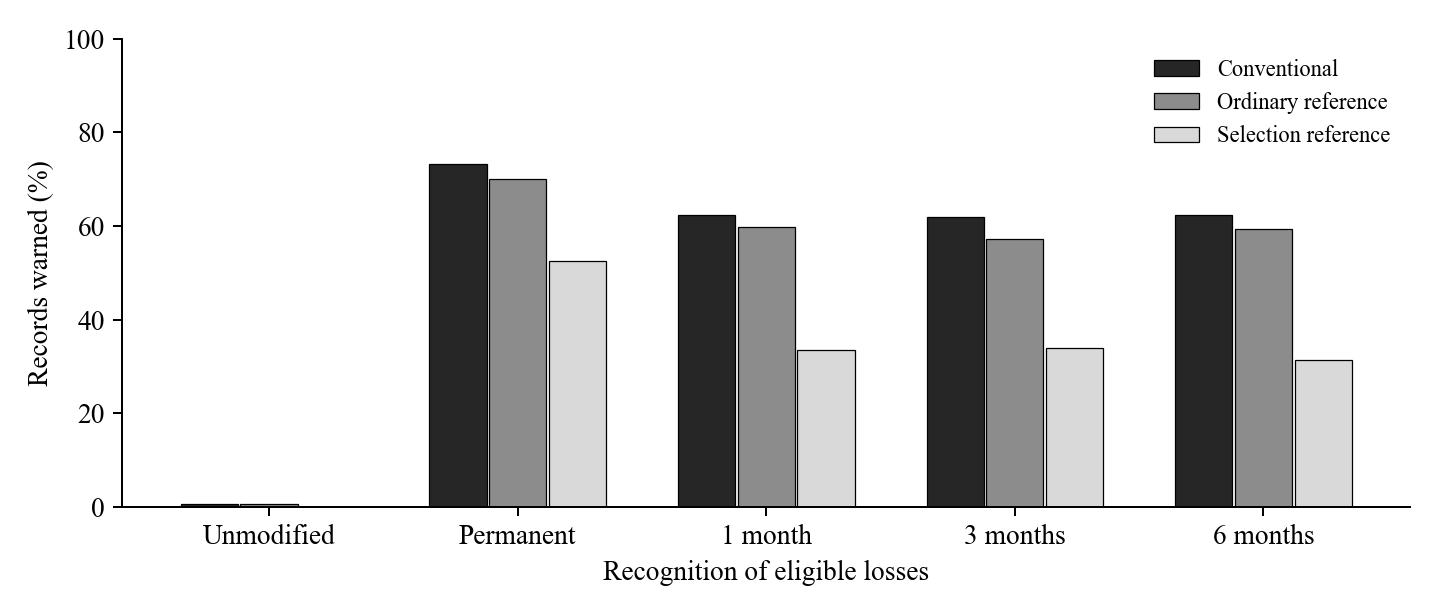
\includegraphics[width=0.97\linewidth]{figures/reporting_tradeoff.png}\end{center}

\textbf{The main tradeoff.} Recognising a hidden loss three months later reduces conventional detection from 142/194 under permanent concealment to 120/194. Detection here means the fraction of altered records that warn; 119 of these 120 warnings are newly triggered. The selection rule warns on 66/194, or 34.0\%, all new. The ordinary calibrated rule detects 111/194. Removing a baseline warning has a substantial detection cost in this experiment.

Joint calendar-block resampling gives a conditional 95\% range of \textbf{29.9\%--44.3\%} for the three-month selection-rule detection rate. With only half of eligible losses hidden, the same rule averages 7.35\% detection across 100 policy draws. This is variation on the same observed records. The funded three-month selection result is 55/194; forced-value-weighted spread and funded results are 99/194 and 95/194. Selection-reference detection remains below conventional detection by varying amounts; the ordinary rule is not uniformly less sensitive than the conventional rule.

\newpage
\subhead{4. Can diversification reach Fund X's performance range?}
This is a separately labelled exploratory extension, added after the individual-factor results showed a performance gap. It uses the same 194 factors, with weights fixed using only 2005--2016 returns, and evaluates the resulting portfolios over 2017--2025. It does not shift returns upward to make them resemble Fund X.

Three rules are used: equal notional weights; weights inversely proportional to calibration-period volatility; and maximum calibration Sharpe, with nonnegative weights summing to one, a 5\% cap per factor, and a covariance estimate halfway between the sample covariance and its diagonal. The factor catalogue and data vintage remain retrospective. No calibration cutoffs from the individual-factor experiment are applied to these combinations.

\subhead{Why the cash convention matters}
The source long--short series is a stock-return spread. Treating it as an ordinary fully invested fund return and subtracting the risk-free rate again would change its economic meaning. The primary analysis therefore uses the spread directly. The funded sensitivity assumes one unit of investor equity, one unit long and one unit short, with cash collateral earning the risk-free rate. Its reported return is $r_f+LS$, gross of all implementation costs. This is an explicit financing assumption, not an observed NAV.

For funded returns define $h_0=\bar r/s(r)$, the zero-threshold ratio used in the normal-loss calculation, and $h_e=\overline{r-r_f}/s(r-r_f)$, the usual monthly excess-return Sharpe ratio. They answer different questions. Cash interest can lift $h_0$ substantially for a quiet strategy without producing the same increase in risk-adjusted investment performance.

\begin{center}
\small
\begin{tabular}{lrrrrrr}
\toprule
Funded record & Mean & SD & $h_0$ & $h_e$ & Bias & $p_N$ \\
\midrule
Equal notional & 0.461\% & 0.761\% & 0.605 & 0.350 & 1.88 & 0.427 \\
Inverse volatility & 0.362\% & 0.561\% & 0.645 & 0.300 & 2.22 & 0.295 \\
Maximum calibration Sharpe & 0.431\% & 0.514\% & 0.839 & 0.473 & 2.25 & 0.492 \\
Fund X & 3.445\% & 4.068\% & 0.847 & 0.796 & 12.83 & $<0.00001$ \\
\bottomrule
\end{tabular}
\end{center}
\note{Original-construction combinations, plus Fund X, all over the same 108 months. Mean and SD are monthly. Bias means the bias ratio; $p_N$ is the fitted-normal loss-count probability. Both Sharpe-type ratios are monthly and are not annualised. Fund X is net reported; combinations are gross reconstructed returns.}

The funded maximum-calibration-Sharpe combination has $h_0=0.839$, close to Fund X's 0.847. However, its mean return is only \textbf{0.431\% a month}, versus Fund X's \textbf{3.445\%}, and its excess-return Sharpe is \textbf{0.473 versus 0.796}. It is not a comparable economic performance record. Its calibration-period excess Sharpe was 2.011, illustrating a large subsequent fall despite the fixed-weight evaluation.

Its bias ratio of 2.25 triggers the conventional bias screen, while its normal-count $p=0.492$ does not. Equal-notional funded diversification triggers neither screen. The forced-value-weighted maximum-Sharpe combination has excess Sharpe 0.079 and bias ratio 2.41. Across the six combination rules and weighting constructions, all spread versions are unflagged; three funded versions trigger the bias rule.

\textbf{Interpretation.} Transparent portfolio construction can produce a modest bias-ratio warning, and cash interest can change a screen's appearance. This is useful evidence about financing and the zero threshold. It does not explain Fund X's much larger bias ratio of 12.83, verify its returns, or make the two performance records economically equivalent.

\newpage
\subhead{What this adds to the paper}
The most defensible addition is an empirical comparison of the decisions made by the screens: on transparent post-publication factor histories, after selection among historical performers, and after explicitly reconciled reporting changes. Its strongest result is the cost of making a screening rule stricter. It also shows why cash interest and the distinction between an excess payoff and a funded return matter.

This is stronger than a single Fund X illustration, but it does not establish a substantial new statistical method. Bollen and Pool (2012) study return flags and fraud risk; Jorion and Schwarz (2014) show alternative explanations for zero-return discontinuities. Van Vuuren and van Vuuren (2022) already apply bias ratios and return moments to hedge-fund strategy indices and discuss warnings alongside good performance. The increment here is the \emph{measured magnitude} of selection, financing and detection effects under fixed policies; the existence of a stricter-cutoff tradeoff is itself familiar. Whether that empirical increment is sufficient for \emph{Risk Sciences} remains an editorial judgment.

\subhead{Changes to the proposed hypotheses}
\textbf{High Sharpe and selection.} The 108-month factor evidence does not support a broad statement that higher Sharpe necessarily causes more warnings. Only the highest Sharpe quintile has a warning, but it is one event; the best full-pool record does not warn. Shorter windows show larger, uneven effects. Sparse descriptive logit fits cannot support reliable coefficient or significance claims here.

\textbf{Calibration and detection.} The proposed claim that calibration lowers false alarms without materially reducing detection is contradicted by the specified three-month experiment. Report the 120/194 to 66/194 change, and retain the held-out 9.4\% sensitivity failure. Use ``warning on an unmodified reconstructed strategy'', not a verified false-positive rate for honest managers.

\textbf{Smoothing.} A one-lag weighted average applied to both gains and losses increases mean first-order autocorrelation from 0.055 to 0.343, 0.528 and 0.340 at weights 0.25, 0.50 and 0.75. Conventional warnings are 7, 4 and 4 out of 194, versus 1 originally. Neither effect is monotone across the full range. Serial dependence alone does not identify deliberate concealment.

\textbf{The Fund X comparison.} Keep Fund X as motivation and a test case. The individual factors do not cover its performance range, and the close funded-combination ratio relies substantially on cash interest. The experiments do not establish that spectacular returns are authentic, fraudulent, or beyond meaningful return-based investigation.

\subhead{A practical implication an investor could use}
A warning should prompt reconciliation of the reported return definition, financing, fees, valuation and timing, rather than an allegation. A quiet screen should not reduce the need to reconcile NAVs and cash flows. If a manager can recognise a small loss later, the investment P\&L can remain unchanged while the monthly record looks different. Raising cutoffs to accommodate historical-winner selection makes that problem harder to detect. Report the ordinary and selection-reference results together instead of replacing the original result with the more favourable one.

\subhead{Sources and reproducibility}
\note{Chen and Zimmermann (2022), \emph{Open Source Cross-Sectional Asset Pricing}, Critical Finance Review 11(2), 207--264; official \href{https://www.openassetpricing.com/data/}{data library} and \href{https://huggingface.co/datasets/OpenSourceAP/CrossSection/tree/dd1054254c4501776432caa6d7ce5ecd9586f6a9}{pinned October 2026 release}. Risk-free data: \href{https://mba.tuck.dartmouth.edu/pages/faculty/ken.french/Data_Library/f-f_factors.html}{Kenneth French Data Library}; source changes in June 2024. Bollen and Pool (2012), \href{https://doi.org/10.1093/rfs/hhs085}{Suspicious Patterns in Hedge Fund Returns and the Risk of Fraud}; Jorion and Schwarz (2014), \href{https://doi.org/10.1016/j.jfineco.2013.10.001}{Are Hedge Fund Managers Systematically Misreporting? Or Not?}; van Vuuren and van Vuuren (2022), \href{https://doi.org/10.1177/21582440221097925}{Detecting Investment Fraud Using the Bias Ratio}.}

\note{The accompanying workbook contains every strategy, observed selection result, calibration and held-out resample summary, reporting policy and sensitivity. Matching source data, frozen designs, exact cutoffs, scripts and independent numerical checks are retained in Assignment 9. Wide and long source files agree exactly; return dates, units and accounting identities were checked, and the principal selection and reporting results were reproduced separately.}
\end{document}
